% ====================================================================
%+
% SECTION:
%    sn.tex
%
% CHAPTER:
%    transients.tex
%
% ELEVATOR PITCH:
%
%-
% ====================================================================

\section{Supernovae as Transients}
\def\secname{\chpname:SNtransients}\label{sec:\secname}

\credit{fedhere}

Supernovae (SNe) represent the final dramatic stages of life of many
stars. The term SN we covers a diverse set of phenomena: explosion of
low mass stars in binary systems, thermonuclear SN or SN Ia (also
discussed in \autoref{sec:supernovae}), and explosion of high mass stars,
Core collapse (CC) SNe, and even terminal explosions of more exotic
systems, yet to be understood, like Super Luminous SNe
(SLSNe). Phenomenologically, the observable of the explosion are
themselves diverse. The transient duration ranges between weeks,
months, even years. The electromagnetic energy radiated ranges between
$\sim0.1$ (faintest CC SNe), to $\sim1$ (SN Ia) and $\sim100$ (SLSNe)
$\times 10^{49}$ erg, corresponding to absolute magnitudes at peak
ranging between $\sim-19$ and $\sim-22$.

LSST's contribution to SNe studies can can be substantial. Synoptic
surveys such as SDSS, SNLS, PTF, PanSTARRS have revolutionized our
understanding of SN over and over again, exposing their diversity,
and revealing different progenitor channels. LSST's first crucial
input will be discovery: the normal type Ia SN rate out to redshift
$z=1$ is estimated to be $\sim200 ~(\mathrm{sq. deg.})^{-1}$ per
year\footnote{\url{http://www.lsst.org/sites/default/files/docs/Wood-Vasey_086.11.pdf}},
and SN~Ia represent only about 1/4 of all SN
events~\citep{Li11b}: tens of millions of stars will explode
within the LSST footprint every year. The key questions concerning
LSST SN science are:
\begin{itemize}
\item
LSST's SN discovery power,
\item
LSST's discrimination power,
\item
the quality of the statistical sample over time.
\end{itemize}
The first and second topic are \emph{time sensitive}, while the latter
is not, although it is interesting to understand the pace at which a
science question can be advanced in the life time of LSST.

{\bf \emph{Discovery:}} the SN~Ia discovery is rate is a standard LSST time-domain metric: a
fraction of $\sim40\%$ SN~Ia are expected to be discovered pre-peak
luminosity within the standard LSST survey
(e.g. \opsimdbref{db:baseCadence}~Figure~\ref{fig:enigmaEarlySNe}). The
topic of SNe discovery is discussed in further detail in
\ref{sec:supernovae}.

The next step is then {\bf\emph{discrimination}}, and the question we need
to answer, for SNe as well as for most other transients, is: will LSST
photometry allow to distinguish SN from other transients, and to
distinguish the different types of SN? And further: will this be
achievable in time to appropriately direct follow-up efforts? This is
particularly difficult considering that photometric classification
schemes have only achieve modest performances in distinguishing, for
example SN~Ic from SN~Ia. As mentioned earlier in this chapter, the issue
of prompt classification is at the heart of the success of LSST
transient science, but it is too complex to tackle in this chapter,
while LSST's ability to assess whether a new transient is young is discussed
in \autoref{sec:\chpname:transientsAge}.

When a large statistical sample of SNe is generated, LSST's photometry
may allow to set constraints on the diversity of the sample, even as a
standalone survey, without the aid of follow-up efforts.  {\bf Thus
  LSST \emph{alone} can shed light on the diversity within the
  population of SN}, which in turn may constrain the genesis of the
explosion.\footnote{Reliable typing of a SN and redshift determination
  would still require auxiliary data.} For SN~Ia, where the exploding
star is a Carbon-Oxygen (CO) White Dwarf (WD), outstanding questions
that can be answered by an LSST photometric sample include, for
example, what is the percentage of SN Ia that arise from a
\emph{double degenerate} (DD) progenitor system -- a CO WD-WD binary
--, from a \emph {single degenerate} (SD) system -- a WD-Main Sequence
(MS) or WD-Red Giant (RG) binary--, or a \emph{merger} -- a WD-WD
binary with a He and a CO WD. Answering this question would reduce the
scatter in the Hubble diagram if SNe from different progenitors are
shown to require different standardization~\citep{Scolnic2014}. On the
CC~SN side: the diversity of SN sub-classes, and the relationship
between them (is there a phenomenological continuum or actually
distinct classes, e.g. between IIp and IIL, or Ib and IIb?) is yet to
be understood. Exceptionally well studied objects may answer these
questions: individual SN Ia with tight constraints on the progenitor
system show, for example, that both single and double degenerate
progenitors exist (e.g. SN 2011fe, \citealt{Li11}, ~\citealt{Olling15}
and PTF 11kx, \citealt{Dilday12}). However, a statistical sample is
needed to set constraints on populations.

Thus the technical question to be answered is: how much detail can be
sacrificed in favor of sample size without compromising diagnostic
power? And the diagnostic power relies on color and sampling: thus
what is the trade-off between cadence in the same filter, and
observations in different filters. Specifically, transients can be
distinguished early from two photometric characteristics: rise time
and color. There is a tension between these observables, as discussed
in Section~\ref{sec:\chpname:transientsAge}. Obtaining colors relies
of course on obtaining photometry in different bands as close as
possible to \emph{simultaneously}. However, assessing the rise slope
is best done with a single filter, so prompt characterization also
needs multiple epochs within a night, although separated by at least a
few hours, in the same filter, as observing with different
filters it is impossible (or very hard) to separate shape from
color. Colors allow to learn a lot about the
statistical sample: as long as the epoch of peak is reliably assessed
coadded light curves can be studied, which is the goal of the analysis
that follows.

\subsection{Distinguishing progenitor scenarios}

In this chapter we envision and design a SN related metric that works
on a large sample (months, to years of LSST data) and assesses the
ability to characterize the contribution of SNe with specific features
to the global population: as a test case we will use the presence of
an early blue excess for SN type Ia, signature of interaction with a
companion, and thus of a SD progenitor. Equivalently, the presence of
an early blue excess in CC~SNe could be assessed, the signature of shock
breakout, which directly measures the radius of the progenitor
star. The \emph{figure of merit} for this science case is the time
within the survey required to achieve a sufficiently large sample of
SNe satisfying proper quality criteria to enable us to distinguish
populations with different contribution from DD and SD progenitors.
To do this we rely on simulations of the observables of the population
for different sample sizes, and on the \texttt{transientAsciiMetric}
to determine the detectability of interacting, and non-interacting
SNe. We are developing a metric (\texttt{colorGapMetric}) to assess
the gap between of detections in 2 filters. In the meantime we rely on
the estimated of the gap between observations in a single filter, and
in any filters (see~\autoref{sec:\chpname:analysis}).

We simulate interacting SNe from the Nugent templates \citep{Nugent02}
injecting the angle dependent effects of interaction with a companion
as simulated by \citep{Kasen10}, for a $2~M_\odot$ and a $6~M_\odot$
MS companion stars, and a $1~M_\odot$ RG companion, following the
procedure of ~\citep{Bianco11}. We create synthetic progenitor
populations with a fraction of single degenerate progenitor systems
$0.05 \leq f_\mathrm{SD} \leq 0.6 $ in 0.05 intervals, and random lines of
sight with respect to the binary's geometry. One such lightcurve, with
maximal interaction effects, is shown in \autoref{fig:kasenlc}, also
indicating how it may be observed by LSST. For each population we
simulate the observation of colors by selecting random epochs with a
granularity of 1 day within the first 10 days after explosion, and
subtracting the magnitude in different filters at the same epoch
$\pm~1$~day for each SN, and we include the effects of observational
noise by generating datapoints from a draw within a Gaussian
distribution centered at the color measured in the previous step and
with standard deviation $\sigma_\mathrm{pop} = 0.1$, 0.3, and 0.5.  We
generate populations of $N_\mathrm{pop}=100$,~1000,~10000 $z~=~0.5$ SNe,
observed in $g'-r'$, as a representative case. Because the effect is
heavily chromatic, and it dissipates becoming essentially negligible
by $r$ band, $u'-i'$ gives the most leverage. However $g'$ and $r'$
are the best observed LSST bands in most cadences. An extension of
this work should then consider $g'-r'$, $u'-r'$, $g'-i'$, and $u'-i'$.

\begin{figure}[hbt]
\centerline{
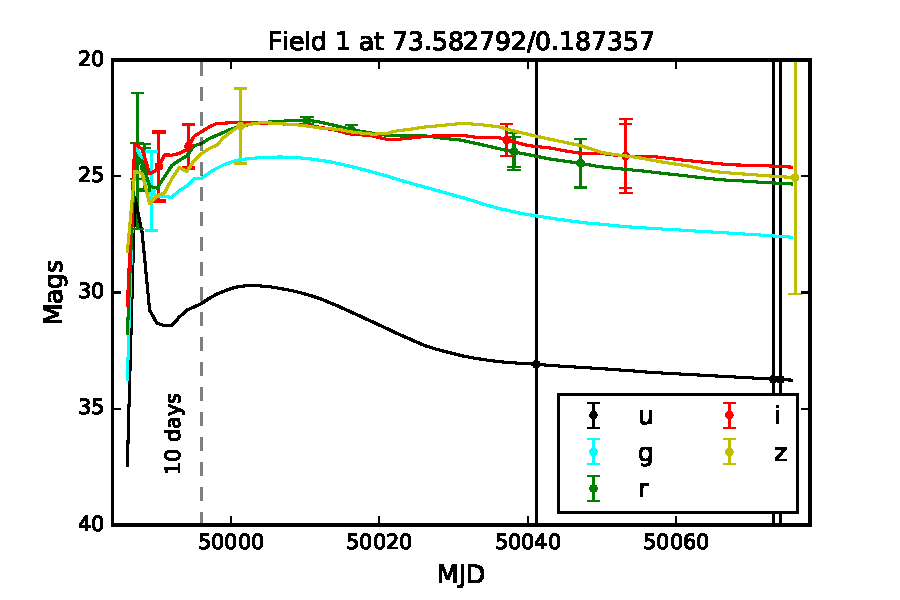
\includegraphics[width=0.6\textwidth]{figs/transients/LSST_Kasen_lcv0.pdf}
}
\caption{ A normal SN Ia lightcure at z=0.5 showing interaction with a
  RG companion as seen from the most favorable viewing angle: the
  effect of interaction as simulated by \citet{Kasen10} is added on
  top of a lightcurve simulated from the \citealt{Nugent02}
  templates. The data points represent one possible set of LSST
  observations of this transient, obtained by running the
  \texttt{transientAsciiMetric}.  This particular event is detected in
  $g'$, $r'$, and $i'$ within the first 10 days.}
\label{fig:kasenlc}
\end{figure}

We perform Kolmogorov-Smirnoff ($KS$) an Anderson-Darling ($AD$) tests
to evaluate, as a function of $\sigma_\mathrm{pop}$ and sample size
$N_\mathrm{pop}$, our diagnostic power. In \autoref{tab:SNprogenitors}
we report the ability to distinguish a population with a $f_\mathrm{SD} > x$ from
$f_\mathrm{SD}=0.05$; the number reported is the SN~Ia fraction from
SD progenitors that can be distinguished at a $p\mathrm{-value}~\leq
~0.05$.

\begin{table}
\begin{center}
  %\begin{tabular}{ c | c| c| c | c | c| c| c | }
  \begin{tabular}{ c | c| c| c |  }
$g-r$&\bf{$N_\mathrm{pop}$=100}&\bf{$N_\mathrm{pop}$=1,000}&\bf{$N_\mathrm{pop}$=10,000}\\%& $g-i$&\bf{$N$=100}&\bf{$N$=1,000}&\bf{$N$=10,000} \\
  \hline
 \bf{$\sigma_\mathrm{pop} = 0.5$}&  -  & 0.2 & 0.1 \\%& &  -  & -  &  0.2 \\
 \bf{$\sigma_\mathrm{pop} = 0.35$}&  - & 0.2 & 0.1 \\%& &  -  & 0.2 & 0.1 \\
 \bf{$\sigma_\mathrm{pop} = 0.1$}& 0.2 & 0.1 & 0.1 \\%& & 0.4 & 0.1 & 0.1 \\
%&&&&&&&\\ $u-i$&\bf{$N$=100}&\bf{$N$=1,000}&\bf{$N$=10,000} & $u-r$&\bf{$N$=100}&\bf{$N$=1,000}&\bf{$N$=10,000}\\
% \bf{$\sigma_\mathrm{pop} = 2.0$}&  -  & -  &  0.2 & &  -  & -  &  0.2 \\
% \bf{$\sigma_\mathrm{pop} = 1.0$}&  -  & 0.2 & 0.1 & &  -  & 0.2 & 0.1 \\
% \bf{$\sigma_\mathrm{pop} = 0.5$}& 0.4 & 0.1 & 0.1 & & 0.4 & 0.1 & 0.1 \\

 \hline
  \end{tabular}
  \caption{Fraction of single degenerate (SD) SN~Ia in a sample of $z~=~0.5$ SNe that can be distinguished from a population with 95\% double degenerate (DD) and 5\% SD SNe~Ia, for a given noise level ($\sigma_\mathrm{pop}$) and number of observations ($N$).}
\label{tab:SNprogenitors}
\end{center}
\end{table}

At this point we can evaluate how long it will take for a given LSST
cadence to obtain a sufficient number of observations in the 2 desired
bands, separated by less than 1 day, that pass the SNR requirements.
This should be done in a full Monte Carlo simulation, injecting
lightcurves with the proper lightcurve shape at the proper rate.  Note
that, because the early lightcurves of interacting SD SN~Ia are
brighter, they should be more easily detected. However at this stage we
can take some shortcuts. \emph{First shortcut}: we evaluate the
relative observability of SNe with excess, and SNe without excess at
$z~=~0.5$ and adjust the number of detections according to
the injected ratio.  The relative detectability can be assessed with
the \texttt{transientAsciiMetric}, which allows us to see how OpSims
recovers observations of transients with realistic shapes. We conclude
that for RG-WD progenitors the detectability is enhanced by $\sim50\%$ in
 $g'$ compared to SD progenitors, and slightly less in $r'$.

Then we extract from the \texttt{transientAsciiMetric}, the number of
\emph{color observations}, i.e. observations in 2 bands within 1 day
of each other, each fulfilling our SNR requirement for the color for
3-, 6-, and 12 months of survey in year 1. The SNR requirement is 
translated into a requirement on each
observation of $\mathrm{SNR} >
\frac{1.0}{\sqrt{2.0}~\sigma_\mathrm{pop}}$.

With the goal of distinguishing a SD contribution of 10\% to the SN Ia
population to a three-siga level ($p$-value <0.05), we need more than
1000 detections, in 2 filters within 1 day, and a
$\sigma_\mathrm{pop}<0.35$ \autoref{tab:SNprogenitors}. But the pairs
of observations we recovered at the previous step are within the first
10 days but with any gap in time. \emph{Second shortcut}: To include
the constraint that the detections should be within 24 hours we refer
to the \texttt{InterNightGapsMetric}, which is plotted in
~\autoref{fig:enigmaGapAll}.  For the \opsimdbref{db:baseCadence} we
estimate $~\sim10\%$ of the observation are revisited within a
night. With the assumption that this is likely to happen in two
different filters, which is \emph{non-conservative}, but neglecting
intra-night observations that may happen in the two different filters,
which is a \emph{conservative} assumption our numbers drop by a factor
10.

With all these assumptions standing, we find that
 that only 3  months of survey are sufficient to provide a useful,
sufficiently large and high SNR sample for our purpose, and improve on
the findings on this topic that were achieved with SDSS~II~\citep{Hayden2010}, and 3 years
of SNLS data~\citep{Bianco11} with \opsimdbref{db:baseCadence}! With our assumotions, 3 month of survey are just enough to reach the goal for 
\opsimdbref{db:NEOswithVisitTriplets}. Although the \opsimdbref{db:NEOswithVisitTriplets} requires three visits, thus increasing the timeline for inter-night observations, it does not require the observations to be in any specific filters, and with the addition of the third visit within the same night, it increases the typical intra-night gap. It is possible that a detailed investigation of the true \emph{inter-night gap between different filters}, or the addition of a requirement in the cadence that one of the night filter be different than the others (possibly requiring an increased gap between two of the three images to minimize filter changes) would provide valuable data for this kind of studies even faster.

\emph{This exercise demonstrates the power of LSST in collecting large high SNR samples of transients, but we must remind the reader that these conclusion, and generally large sample analysis, rely on having properly identified both the transient class (normal SN~Ia) and the date of maximum! This, once more, highlights the importance of prompt identification and classification: for SN~Ia this likely will limit this work to objects that could be identified spectroscopically, enhancing the importance of follow-up.}


\autoref{fig:sndetect} shows the detection rate for SN~Ia at $z=0.5$
in absence of shock interaction as a function of SNR (obtained by summing in quadrature the errors on $g'$
and $r'$) for 3, 6 months, and a year of
\opsimdbref{db:baseCadence} and \opsimdbref{db:NEOswithVisitTriplets}.
% (ideally I will plot it for the other survey as well tonight) 



\begin{table}
  \begin{tabular}{l|p{6cm}|c|c|p{3cm}}
    FoM & Brief description & {\rotatebox{90}{\opsimdbref{db:baseCadence}}}
	  & {\rotatebox{90}{\opsimdbref{db:NEOswithVisitTriplets}}} & Notes \\
    \hline
    \thesection-1 & \footnotesize{\texttt{SNIaprojenitorMetric},
    \texttt{1,000 detections}}      & 3 & 6 & 
    \footnotesize{Time to collect 1,000 relevant color observations in  years in 3 month intervals.} \\
    \thesection-2     & \footnotesize{\texttt{SNIaprojenitorMetric},
    \texttt{10,000 detections}}      & $>12$ & $>12$ &
    \footnotesize{Time to collect 10,000 relevant color observations in  years in 3 month intervals.}\\
\end{tabular}
\caption{Figures-of-merit (FoMs) for statistical SN Ia progenitor studies to assess the contribution of SD progenitors to the SN Ia population.
}
\label{tab:SummarySNprojs}
\end{table}

\begin{figure}[hbt]
  \centerline{
    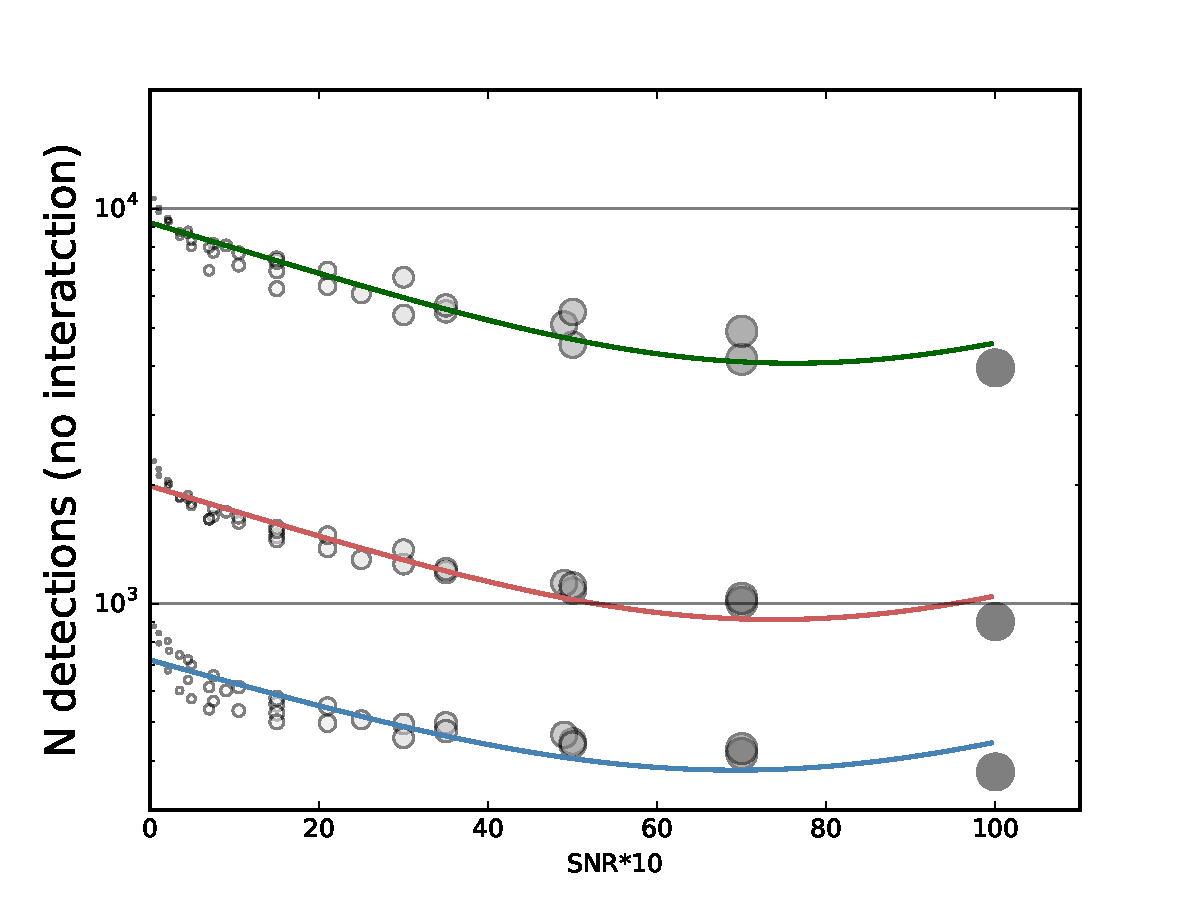
\includegraphics[width=0.6\textwidth]{figs/transients/LSST_Iadetected_wcolor.pdf}
  }
  \caption{
    Normal SN Ia lightcure at z=0.5 detected by the \opsimdbref{db:baseCadence} cadence in 3 months, 6 months, and 1 year, that provide color information useful to constrain the progenitor distribution. Line are third-degree polynomial fits.}
  \label{fig:sndetect}
\end{figure}
